\documentclass[10pt,a4paper]{article}
\usepackage[margin=1.6cm]{geometry}
\usepackage[table]{xcolor}
\usepackage{booktabs}
\usepackage{array}
\usepackage{graphicx}
\usepackage{float}
\usepackage{hyperref}
\setlength{\parindent}{0pt}\setlength{\parskip}{4pt}
\hypersetup{colorlinks=true,urlcolor=blue!70!black,linkcolor=black}
\graphicspath{{../figures/}{figures/}}
\renewcommand{\arraystretch}{1.25}
\definecolor{rowgray}{gray}{0.95}
\newcommand{\q}[1]{\par\colorbox{black!6}{\parbox{\dimexpr\linewidth-2\fboxsep}{\small\textbf{Question:} \textit{#1}}}\par\smallskip}
\newcommand{\good}[1]{\textcolor{green!45!black}{#1}}
\newcommand{\bad}[1]{\textcolor{red!70!black}{#1}}

\begin{document}\sloppy

\begin{center}
{\LARGE\bfseries RAG Assignment: Baseline vs.\ Re-Ranking}\\[8pt]
{\large Hardik Kothari \quad|\quad En.\ No: 2025201046}\\[8pt]
\colorbox{yellow!35}{\textbf{GitHub:} \url{https://github.com/kotharihardik/LMA_Assignment_1_RAG}}\\[4pt]
Notebook: \texttt{RAG\_Assignment.ipynb}
\end{center}

\section*{Setup}
\textbf{Document:} \emph{Bharatiya Nyaya Sanhita, 2023} (Indian criminal code, 102 pages, 358 sections), split into \textbf{504 chunks} of 150 words with 30 words overlap.
I picked it because it has many general rules followed by \emph{Exceptions}, negations (``Nothing is an offence which\ldots'') and sections that share the same words.
\textbf{Bi-Encoder:} \texttt{all-MiniLM-L6-v2} + FAISS inner product (cosine).
\textbf{Cross-Encoder:} \texttt{ms-marco-MiniLM-L-6-v2}.
\textbf{LLM:} \texttt{gpt-oss-120b} via Groq API, temperature 0, same prompt for both pipelines (Llama-3 8B on Ollama froze my 8\,GB laptop).
Pipeline 1 gives the bi-encoder's top 3 of 10 to the LLM; Pipeline 2 re-scores the same 10 with the cross-encoder and gives its top 3.
For every query the \emph{gold chunk} is the chunk containing the clause that actually answers it.

\begin{table}[H]\centering\small
\rowcolors{2}{rowgray}{white}
\begin{tabular}{@{}cll@{}}
\toprule
\textbf{Q} & \textbf{Failure type} & \textbf{Query}\\
\midrule
Q1 & Keyword trap & Is it a crime to buy a stolen mobile phone if I did not know it was stolen?\\
Q2 & Exception & Is it murder if two people get into a sudden quarrel and one kills the other in anger?\\
Q3 & Negation (``except'') & Can a person who commits murder under threat of death escape punishment?\\
Q4 & Negation + role limit & When is a person not allowed to use private defence against a public servant?\\
Q5 & Buried chunk & Is it an offence to harm someone to prevent a bigger harm like a fire?\\
Q6 & Buried chunk & Is it an offence to hurt someone during a sports match?\\
Q7 & Limitation & Is a ten year old child criminally responsible?\\
Q8 & Limitation & Is attempting to commit suicide a crime?\\
\bottomrule
\end{tabular}
\end{table}

%-----------------------------------------------------------------------
\section{Architecture Comparison}
\q{Briefly explain the core difference between a Bi-Encoder and a Cross-Encoder.}

A \textbf{bi-encoder} encodes the query and each chunk \emph{separately} into one vector and scores them by cosine similarity.
Chunk vectors do not depend on the query, so they are computed once and searched very fast.
But the whole chunk is squeezed into one vector before the question is seen, so it mostly captures the \emph{topic}; words like ``except'' or ``not'' barely change it.

A \textbf{cross-encoder} reads query and chunk \emph{together} as one input, so self-attention connects every query token with every chunk token and the model outputs one relevance score.
It can check whether the chunk really \emph{answers} the question, but nothing can be pre-computed: each (query, chunk) pair needs a full forward pass.

%-----------------------------------------------------------------------
\section{Qualitative and Rank Shift Analysis}
\q{Document the rank changes for your failure queries (e.g., Chunk X moved from Rank \#8 $\rightarrow$ Rank \#1).}

\begin{table}[H]\centering\small
\rowcolors{2}{rowgray}{white}
\begin{tabular}{@{}cllcl@{}}
\toprule
\textbf{Q} & \textbf{Gold chunk} & \textbf{Rank change} & \textbf{In Top 3?} & \textbf{Result}\\
\midrule
Q1 & Chunk 417 (Sec 317) & Rank \#6 $\rightarrow$ Rank \#1 & no $\rightarrow$ yes & \good{Restored}\\
Q2 & Chunk 154 (Sec 101, Exc.\ 4) & Rank \#6 $\rightarrow$ Rank \#1 & no $\rightarrow$ yes & \good{Restored}\\
Q3 & Chunk 59 (Sec 32) & Rank \#4 $\rightarrow$ Rank \#1 & no $\rightarrow$ yes & \good{Restored}\\
Q4 & Chunk 63 (Sec 37) & Rank \#5 $\rightarrow$ Rank \#3 & no $\rightarrow$ yes & \good{Restored}\\
Q5 & Chunk 46 (Sec 19) & Rank \#4 $\rightarrow$ Rank \#1 & no $\rightarrow$ yes & \good{Restored}\\
Q6 & Chunk 49 (Sec 25) & Rank \#5 $\rightarrow$ Rank \#1 & no $\rightarrow$ yes & \good{Restored}\\
Q7 & Chunk 46 (Sec 21) & Rank \#2 $\rightarrow$ Rank \#6 & yes $\rightarrow$ no & \bad{Degraded}\\
Q8 & Chunk 302 (Sec 226) & Rank \#7 $\rightarrow$ Rank \#4 & no $\rightarrow$ no & Improved, not enough\\
\bottomrule
\end{tabular}
\end{table}

\begin{figure}[H]\centering
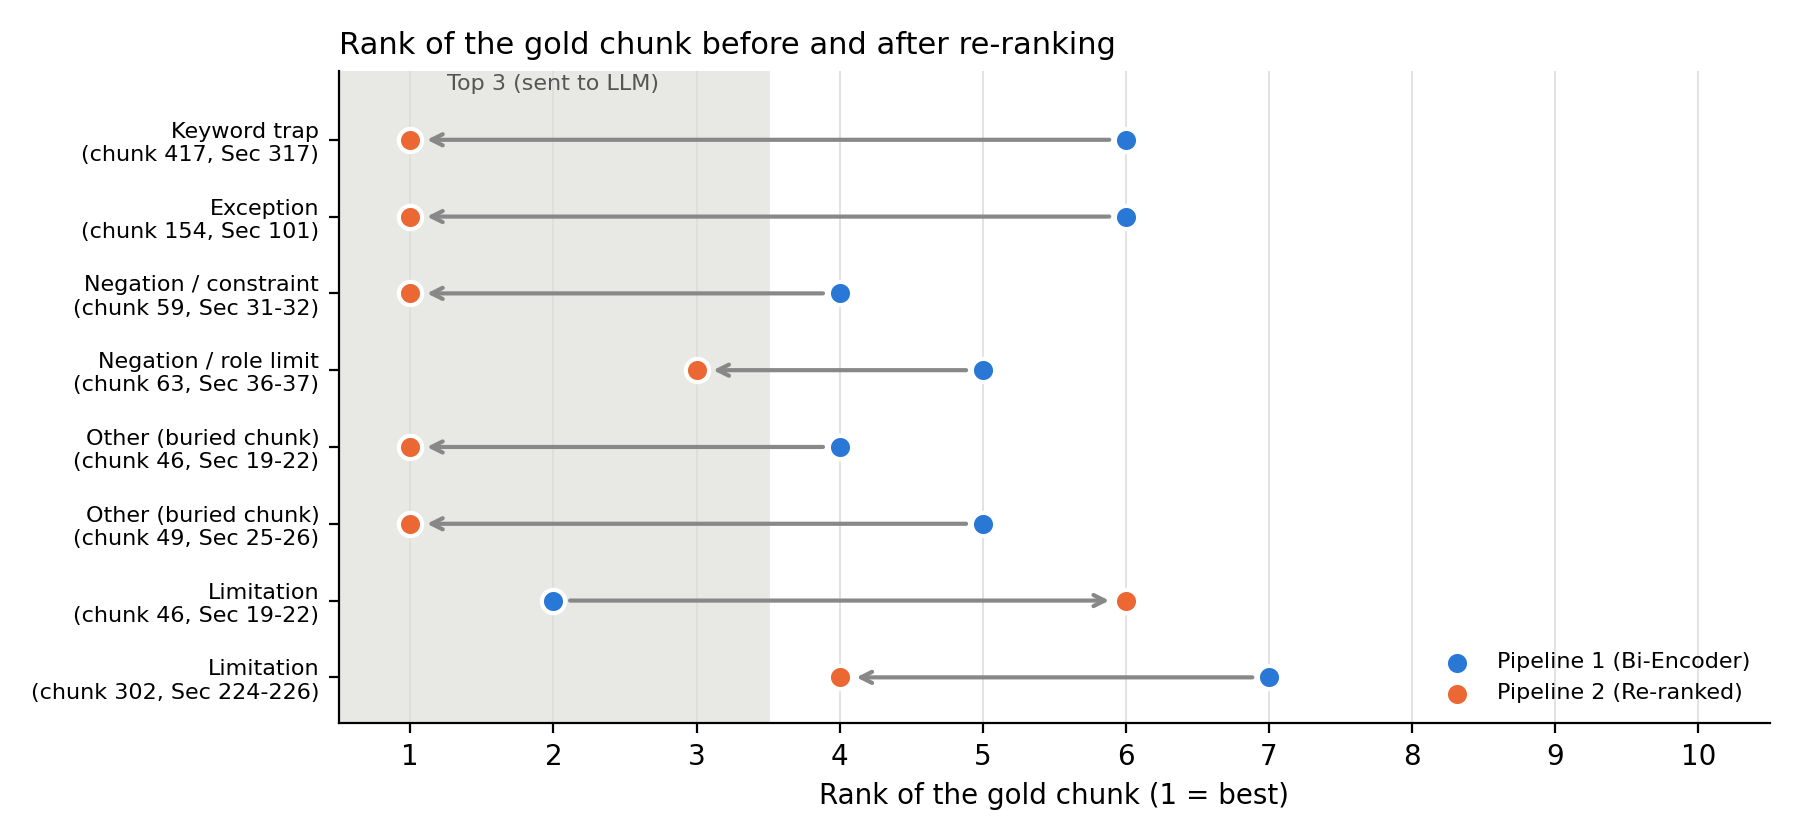
\includegraphics[width=0.78\linewidth]{rank_shift.png}
\end{figure}

\begin{table}[H]\centering\small
\begin{tabular}{@{}lcccc@{}}
\toprule
\textbf{Metric (8 queries)} & \textbf{Hit@1} & \textbf{Hit@3} & \textbf{MRR@10} & \textbf{Mean gold rank}\\
\midrule
Pipeline 1 (Bi-Encoder) & 0.000 & 0.125 & 0.235 & 4.9\\
Pipeline 2 (Re-ranked) & \textbf{0.625} & \textbf{0.750} & \textbf{0.719} & \textbf{2.3}\\
\bottomrule
\end{tabular}
\end{table}

In Q1--Q6 the gold chunk was in the bi-encoder's top 10 but at rank 4--6, so it never reached the LLM.
The cause was topic overlap: for Q1 the top chunks were Sec 303 theft illustrations (same words: stolen, watch, property), and for Q3 they were all about murder punishment.
The cross-encoder moved the gold chunk into the top 3 in all six cases.
(These are hard queries chosen on purpose, not an average case.)

\q{Compare LLM Answer 1 vs.\ Answer 2: Did the baseline generate a hallucination, omit an essential clause, or misstate a rule because the critical chunk sat outside the top 3?}

I checked each answer against the gold clause. A refusal (``context does not contain this information'') counts as an omission, since the answer exists in the Act.

\begin{table}[H]\centering\small
\rowcolors{2}{rowgray}{white}
\begin{tabular}{@{}clll@{}}
\toprule
\textbf{Q} & \textbf{Answer 1 (baseline)} & \textbf{Answer 2 (re-ranked)} & \textbf{Note}\\
\midrule
Q1 & \bad{Omitted clause} & \good{Correct} & A2 gives ``knowing or having reason to believe'' (Sec 317)\\
Q2 & \bad{Misstated rule} & \good{Correct} & A1 used the provocation exception; A2 used Exception 4\\
Q3 & \bad{Omitted clause} & \good{Correct} & A2 states ``Except murder'': threats do not excuse murder\\
Q4 & \bad{Misstated rule} & \bad{Misstated rule} & both read Explanation 1 wrongly, missed Sec 37(1)(a)\\
Q5 & \bad{Omitted clause} & \good{Correct} & A2 gives the necessity exception (Sec 19)\\
Q6 & \bad{Omitted clause} & \good{Correct} & A2 gives the consent rule (Sec 25)\\
Q7 & \good{Correct} & \bad{Omitted clause} & re-ranking pushed Sec 21 out of the top 3\\
Q8 & \bad{Omitted clause} & \bad{Omitted clause} & Sec 226 not in the top 3 for either\\
\midrule
\rowcolor{white}\textbf{Total} & \textbf{1/8 correct} & \textbf{5/8 correct} & hallucinations: 0 and 0\\
\bottomrule
\end{tabular}
\end{table}

\begin{itemize}\setlength\itemsep{1pt}
\item \textbf{Omitted an essential clause: yes, the main failure (5 of 8).} E.g.\ in Q3 the baseline never saw Sec 32, so it could not say that threats do \emph{not} excuse murder.
\item \textbf{Misstated a rule: yes (2 of 8).} In Q2 it reached ``not murder'' but from the wrong exception, because only the general definition was in its context.
\item \textbf{Hallucination: no.} With temperature 0 and a strict ``answer only from context'' prompt, the LLM refused rather than invent a law.
\end{itemize}
Re-ranking is not perfect. In Q4 the gold chunk was only Passage 3 and the LLM still followed the similar text above it.
In Q7 the MS-MARCO model (trained on web search, not law) preferred chunks about offences \emph{involving} children and pushed out the correct one.

%-----------------------------------------------------------------------
\section{Latency Profiling}
\q{Record and tabulate the runtime of the baseline retrieval vs.\ the re-ranking pipeline.}

Apple M2 CPU, single thread. Retrieval times are the mean of 20 runs per query; LLM time is one API call.

\begin{table}[H]\centering\small
\rowcolors{3}{rowgray}{white}
\begin{tabular}{@{}lccccc@{}}
\toprule
 & \multicolumn{3}{c}{\textbf{Retrieval (ms)}} & \multicolumn{2}{c}{\textbf{End-to-end (s)}}\\
\cmidrule(lr){2-4}\cmidrule(l){5-6}
\textbf{Query} & \textbf{Bi-encoder} & \textbf{Re-rank} & \textbf{Pipeline 2} & \textbf{Pipeline 1} & \textbf{Pipeline 2}\\
\midrule
Q1 & 6.8 & 234.6 & 241.3 & 3.06 & 2.03\\
Q2 & 6.9 & 222.1 & 229.0 & 1.20 & 1.27\\
Q3 & 6.5 & 217.5 & 224.0 & 0.66 & 1.02\\
Q4 & 5.7 & 224.4 & 230.0 & 1.22 & 1.23\\
Q5 & 6.3 & 231.9 & 238.1 & 0.71 & 1.12\\
Q6 & 6.0 & 219.7 & 225.7 & 0.59 & 1.00\\
Q7 & 5.9 & 215.0 & 220.9 & 1.01 & 1.07\\
Q8 & 5.8 & 203.5 & 209.4 & 0.65 & 1.01\\
\midrule
\rowcolor{white}\textbf{Mean} & \textbf{6.2} & \textbf{221.1} & \textbf{227.3} & \textbf{1.14} & \textbf{1.22}\\
\bottomrule
\end{tabular}
\end{table}

\begin{figure}[H]\centering
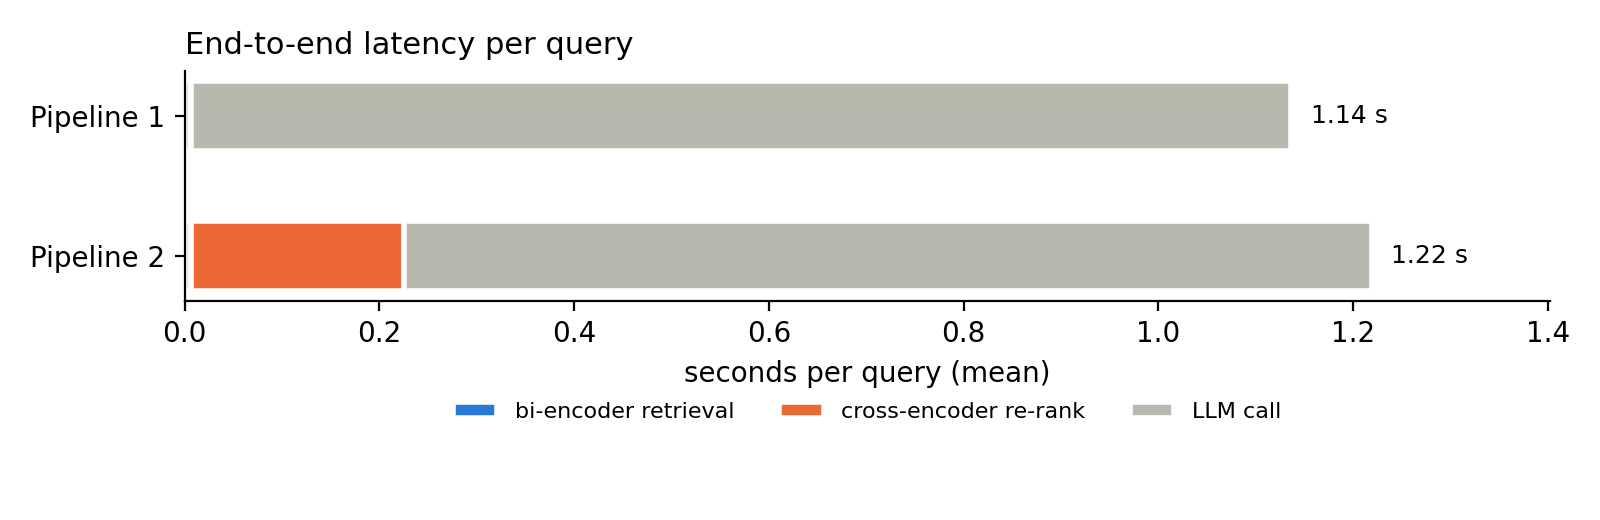
\includegraphics[width=0.58\linewidth]{latency.png}
\end{figure}

Re-ranking makes retrieval about \textbf{36$\times$ slower} (6 ms $\rightarrow$ 227 ms), but end to end the gap is small (1.14 s vs 1.22 s) because the LLM call takes about 1 s.
The LLM time varies between calls, which is why Pipeline 1 is sometimes slower in a single row.

%-----------------------------------------------------------------------
\section{Scaling Question}
\q{Explain why we do not simply run a Cross-Encoder across the entire document collection from the very start.}

The cross-encoder has nothing to pre-compute: its score needs one forward pass over query and chunk \emph{together}, so every new query would need a pass over \emph{every} chunk.
Cost grows linearly with collection size and is paid again for each query.
The bi-encoder does the heavy work offline (chunk vectors once), and per query needs only one encoding plus a fast vector search.

\begin{table}[H]\centering\small
\rowcolors{2}{rowgray}{white}
\begin{tabular}{@{}lcc@{}}
\toprule
\textbf{Collection size} & \textbf{Cross-encoder on all chunks} & \textbf{Two-stage (top 10 only)}\\
\midrule
504 chunks (measured) & 13.3 s & 0.28 s\\
10,000 chunks & $\approx$ 4.4 min & $\approx$ 0.26 s\\
100,000 chunks & $\approx$ 44 min & $\approx$ 0.26 s\\
1,000,000 chunks & $\approx$ 7.4 hours & $\approx$ 0.26 s\\
\bottomrule
\end{tabular}
\end{table}

\begin{figure}[H]\centering
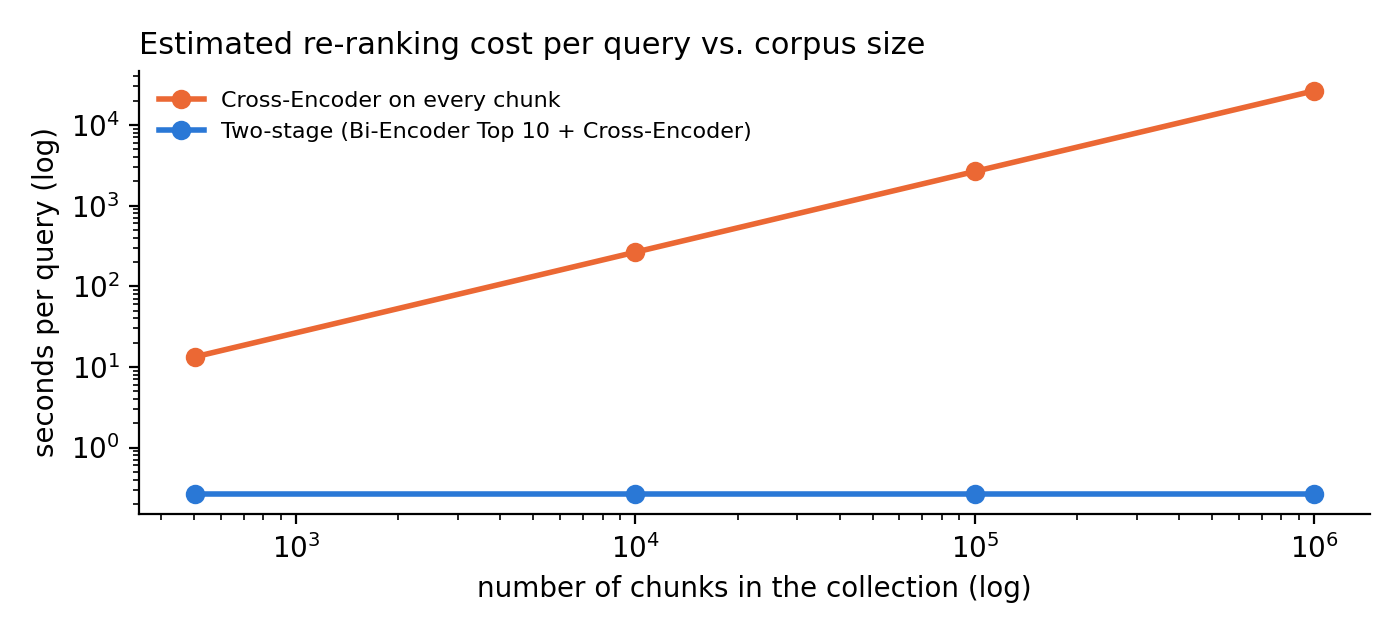
\includegraphics[width=0.48\linewidth]{scaling.png}
\end{figure}

Even for this single Act, cross-encoding everything is about 47$\times$ slower (26.5 ms per pair), and for 5 of 8 queries it gave the \emph{same} top 3 as the two-stage pipeline at about 2\% of the cost.
So the bi-encoder is used as a cheap, high-recall filter and the precise cross-encoder only checks its shortlist.
The trade-off: the re-ranker can only reorder what the bi-encoder found (as in Q8), so a larger pool (top 20--50) would improve recall at some extra latency.

\end{document}
